\documentclass{standalone}
\usepackage{tikz}
\usepackage{tkz-graph}
\usepackage{tkz-berge}

\begin{document}

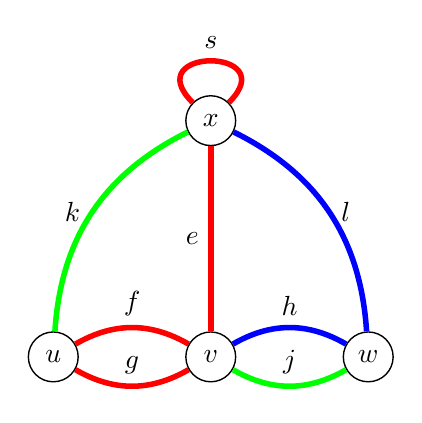
\begin{tikzpicture}
  \SetGraphUnit{2}
  \GraphInit[vstyle=Normal]
  \tikzset{LabelStyle/.style={opacity=0,text opacity=1, black}}
  \Vertex[L=$u$]{A}
  {\tikzset{EdgeStyle/.append style = {red,line width=2pt}}
    \EA[L=$v$](A){B}
    \EA[L=$w$](B){C}
    \SetGraphUnit{3}
    \NO[L=$x$](B){D}
    \Edge[label=$e$,labelstyle=left](B)(D)
    \Loop[dist=1cm, dir=NO, style={-,red}, label=$s$, labelstyle=above](D)
    \tikzset{EdgeStyle/.append style = {bend left}}
    \Edge[label=$f$,labelstyle=above](A)(B)
    \Edge[label=$g$,labelstyle=above](B)(A)
  }
  \tikzset{EdgeStyle/.append style = {bend left}}
  {\tikzset{EdgeStyle/.append style = {blue,line width=2pt}}
    \Edge[label=$h$,labelstyle=above](B)(C)
  }
  {\tikzset{EdgeStyle/.append style = {green,line width=2pt}}
    \Edge[label=$j$,labelstyle=above](C)(B)
    \Edge[label=$k$,labelstyle=left](A)(D)
  }
  {\tikzset{EdgeStyle/.append style = {blue,line width=2pt}}
    \Edge[label=$l$,labelstyle=right](D)(C)
  }
\end{tikzpicture}

\end{document}
